%-----------------------------------------------------------------------------%
\chapter{HASIL PENELITIAN DAN PEMBAHASAN}
%-----------------------------------------------------------------------------%

%
\vspace{4.5pt}
\begin{flushleft}
    \begin{justify}
        \section{Hasil Penelitian}
        \subsection{Penerapan RAD}
        \subsubsection{Pemodelan Bisnis}
        Berdasarkan hasil analisa ditentukan bahwa aplikasi KEBUNQ dirancang untuk satu jenis pengguna. Sehingga tidak terdapat level pengguna pada akses aplikasi.
        Berikut analisa kebutuhan pengguna
        \begin{enumerate}
            \item Pengguna harus melakukan login
            \item Pengguna dapat melihat daftar dan status nyala alat
            \item Pengguna dapat melihat detail alat yang terdiri dari data sensor dan kontrol yang tersedia
            \item Pengguna dapat melakukan kontrol pada alat yang dipilih
            \item Pengguna dapat melakukan setting automatis pada suatu kontrol yang tersedia mode automatisnya\\
        \end{enumerate}
       
        % \begin{enumerate}[label=\alph*.]
        %     \item 
        % \end{enumerate}
        \subsubsection{Pemodelan Data}
        \begin{figure}[ht]
            \centering
            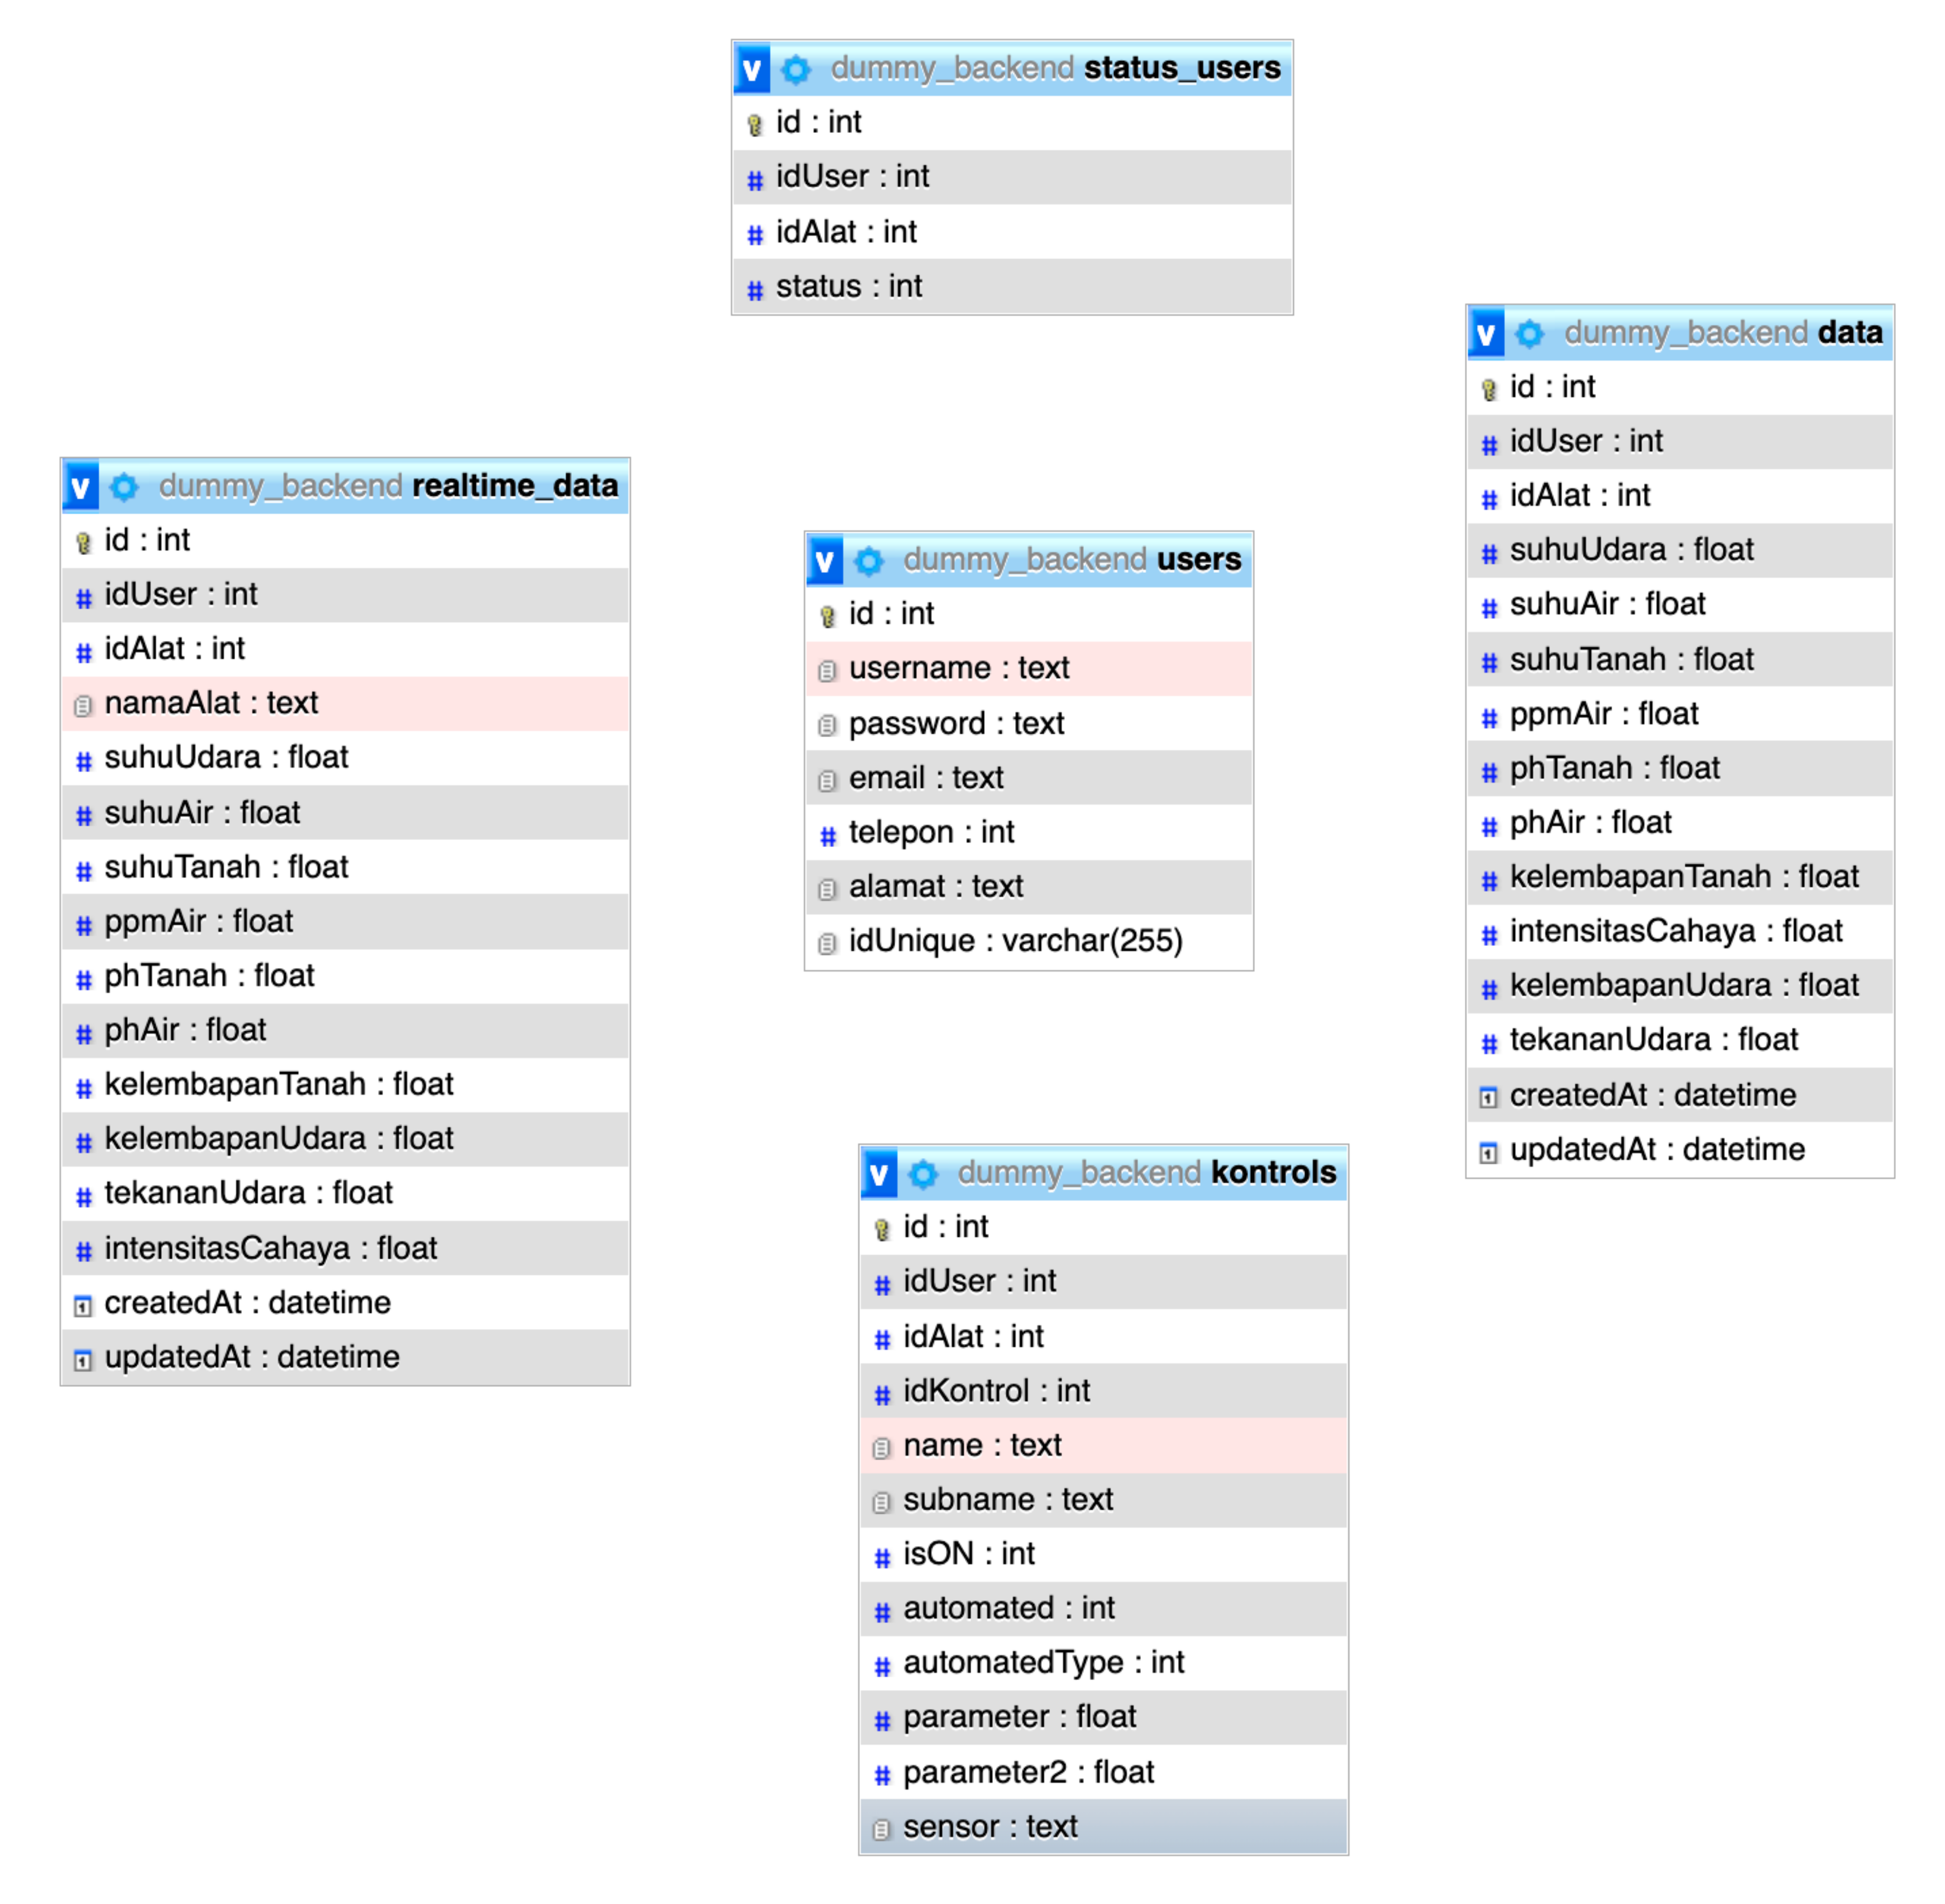
\includegraphics[width=2cm]{images/database.png}
            \caption{Skema Tabel \textit{Database}}
        \end{figure}
\vspace{1cm}
        
        \subsubsection{Pemodelan Proses}
        \begin{enumerate}[label=\alph*.]
            \item \textit{Use Case}
            
            \textit{Use case} perancangan aplikasi mobile KEBUNQ BPP Lampung
            \begin{figure}[ht]
                \centering
                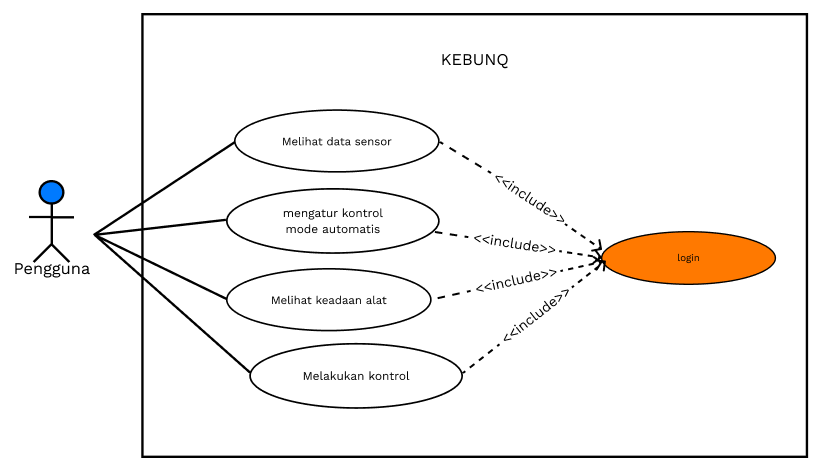
\includegraphics[width=2cm]{images/bab 4/use-case-user.png}
                \caption{\textit{Use Case Diagram}}
            \end{figure}
          \vspace{2cm}
            \item \textit{Sequence Diagram}
            \begin{figure}[ht]
                \centering
                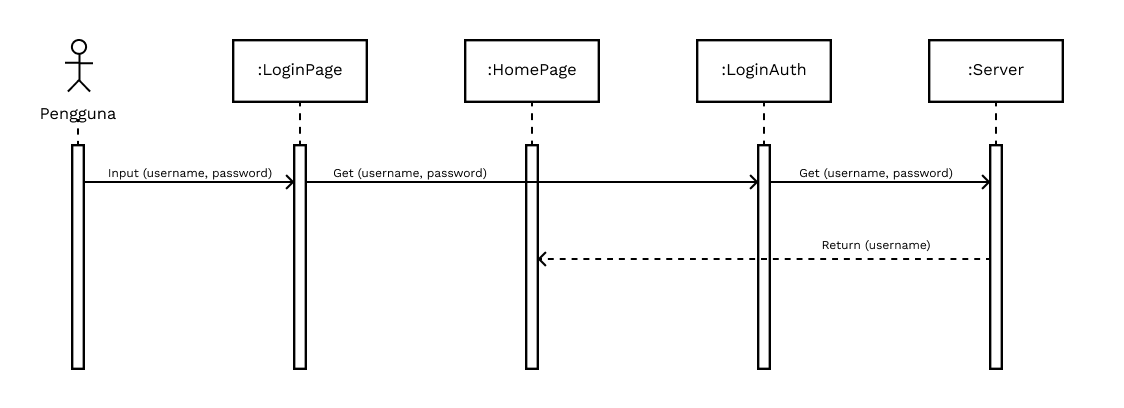
\includegraphics[width=12cm]{images/bab 4/Sequence login.png}
                \caption{\textit{Sequence Diagram Login}}
            \end{figure}
            \begin{figure}[ht]
                \centering
                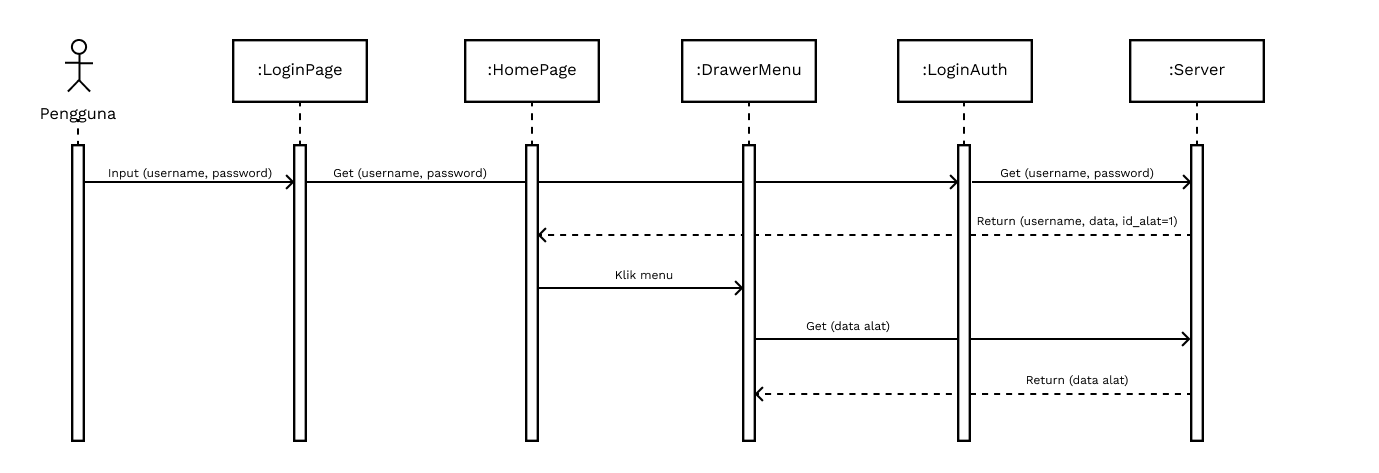
\includegraphics[width=12cm]{images/bab 4/buka menu alat.png}
                \caption{\textit{Sequence Diagram} Melihat Menu / Alat}
            \end{figure}
            \begin{figure}[ht]
                \centering
                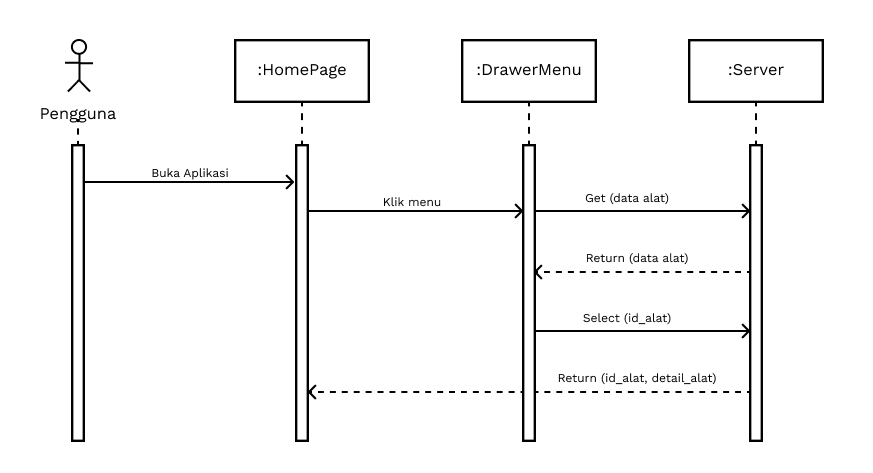
\includegraphics[width=10cm]{images/bab 4/Sequence buka detail alat.png}
                \caption{\textit{Sequence Diagram} Melihat Detail Alat}
            \end{figure}

            \begin{figure}[ht]
                \centering
                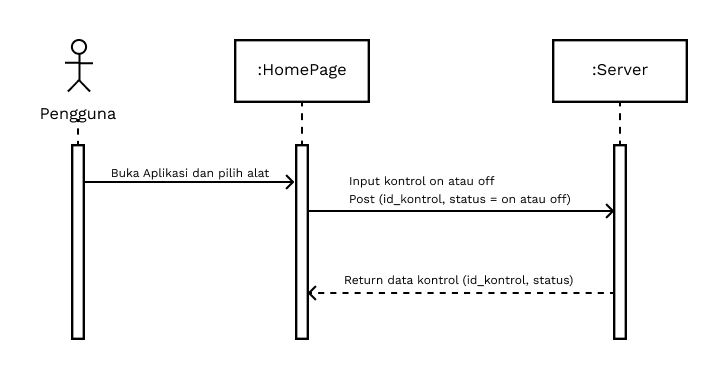
\includegraphics[width=11cm]{images/bab 4/Sequence kontrol.png}
                \caption{\textit{Sequence Diagram} Melakukan Kontrol}
            \end{figure}
            \vspace{2cm}
            \begin{figure}[ht]
                \centering
                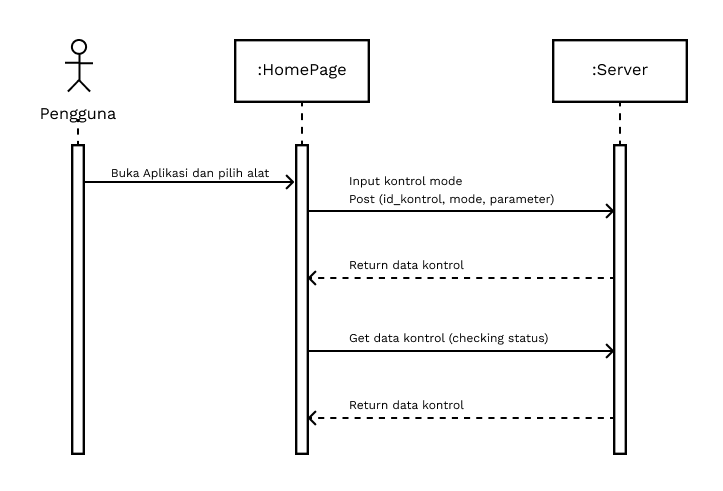
\includegraphics[width=10cm]{images/bab 4/Sequence kontrol Auto.png}
                \caption{\textit{Sequence Diagram} Melakukan Kontrol Automatis}
            \end{figure}
            \end{enumerate}
            \vspace{10cm}
        \subsubsection{Pembuatan Aplikasi}
        Dalam proses pembuatan aplikasi peneliti melakukan 3 pengerjaan (1) Perancangan desain layout \textit{User Interface}, (2) Pembuatan \textit{assets} mencakup logo aplikasi, ikon sensor, dan ilustrasi kontrol, dan (3) Pengerjaan pembuatan aplikasi menggunakan \textit{framework} Flutter dengan bahasa pemrograman Dart
        \begin{enumerate}
            \item Perancangan Desain Layout \textit{User Interface}
        \end{enumerate}
        \subsubsection{Pengujian dan Pergantian}


        \section{Uji Lapangan}

    \end{justify}




    
    \subsection{Data Hasil Observasi}
\vspace{5cm}
\begin{figure}[ht]
	\centering
	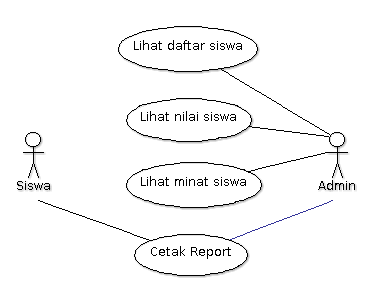
\includegraphics[width=10cm]{images/UseCaseDiagramSistemSaatIni}
	\caption{Gambar Observasi}
\end{figure}
Peneliti mengamati kebutuhan sensor dan kontrol yang diperlukan petani untuk diaplikasikan pada lahannya. 
% \caption{Gambar Observasi}
    \section{Analisis Hasil Penelitian}

\end{flushleft}

\newpage